\chapter{Diseño del protocolo de control In-Band}
\label{ch:analisis}

En este capítulo, se abordará una fase fundamental del proyecto, centrada en el diseño de un protocolo de control In-Band para la gestión de redes. En este capítulo, se realizará un exhaustivo análisis de soluciones anteriores basadas en el enfoque In-Band, donde se explorarán diferentes propuestas y se evaluarán sus fortalezas y debilidades.\\
\\
El objetivo principal será definir las funcionalidades básicas que debe poseer el protocolo de control In-Band, considerando los requisitos específicos del proyecto y las necesidades de los entornos de redes actuales. Se examinarán aspectos clave, como la capacidad de establecer una conexión entre los nodos de la red y el controlador, el manejo eficiente del plano de datos para la transmisión de información de control y la escalabilidad para adaptarse a entornos de redes heterogéneas y de gran tamaño. Además, se proporcionará una explicación detallada del funcionamiento del protocolo diseñado, describiendo los diferentes componentes, los mensajes intercambiados entre nodos y controlador, así como los procedimientos de configuración y gestión de la red. Se analizarán las decisiones de diseño tomadas y se justificarán en base a los objetivos del proyecto y las características de los entornos de redes abordados.Por último, se tomará una decisión sobre la plataforma más adecuada para la implementación del protocolo de control In-Band. Se evaluarán diferentes opciones, considerando factores como la disponibilidad de herramientas y tecnologías relevantes, la compatibilidad con los requisitos del proyecto y la viabilidad de su implementación en entornos reales.

%%%%%%%%%%%%%%%%%%%%%%%%%%%%%%%%%%%%%%%%%%%%%%%%%%%%%%%%%%%%%%%%%%%%%%%%%%%%%%%%%%%%%%%%%%%%%%%%%
\section{Protocolo In-Band}
\label{sec:ana_inband}

iotorii hackmd




\begin{figure}[ht!]
    \centering
    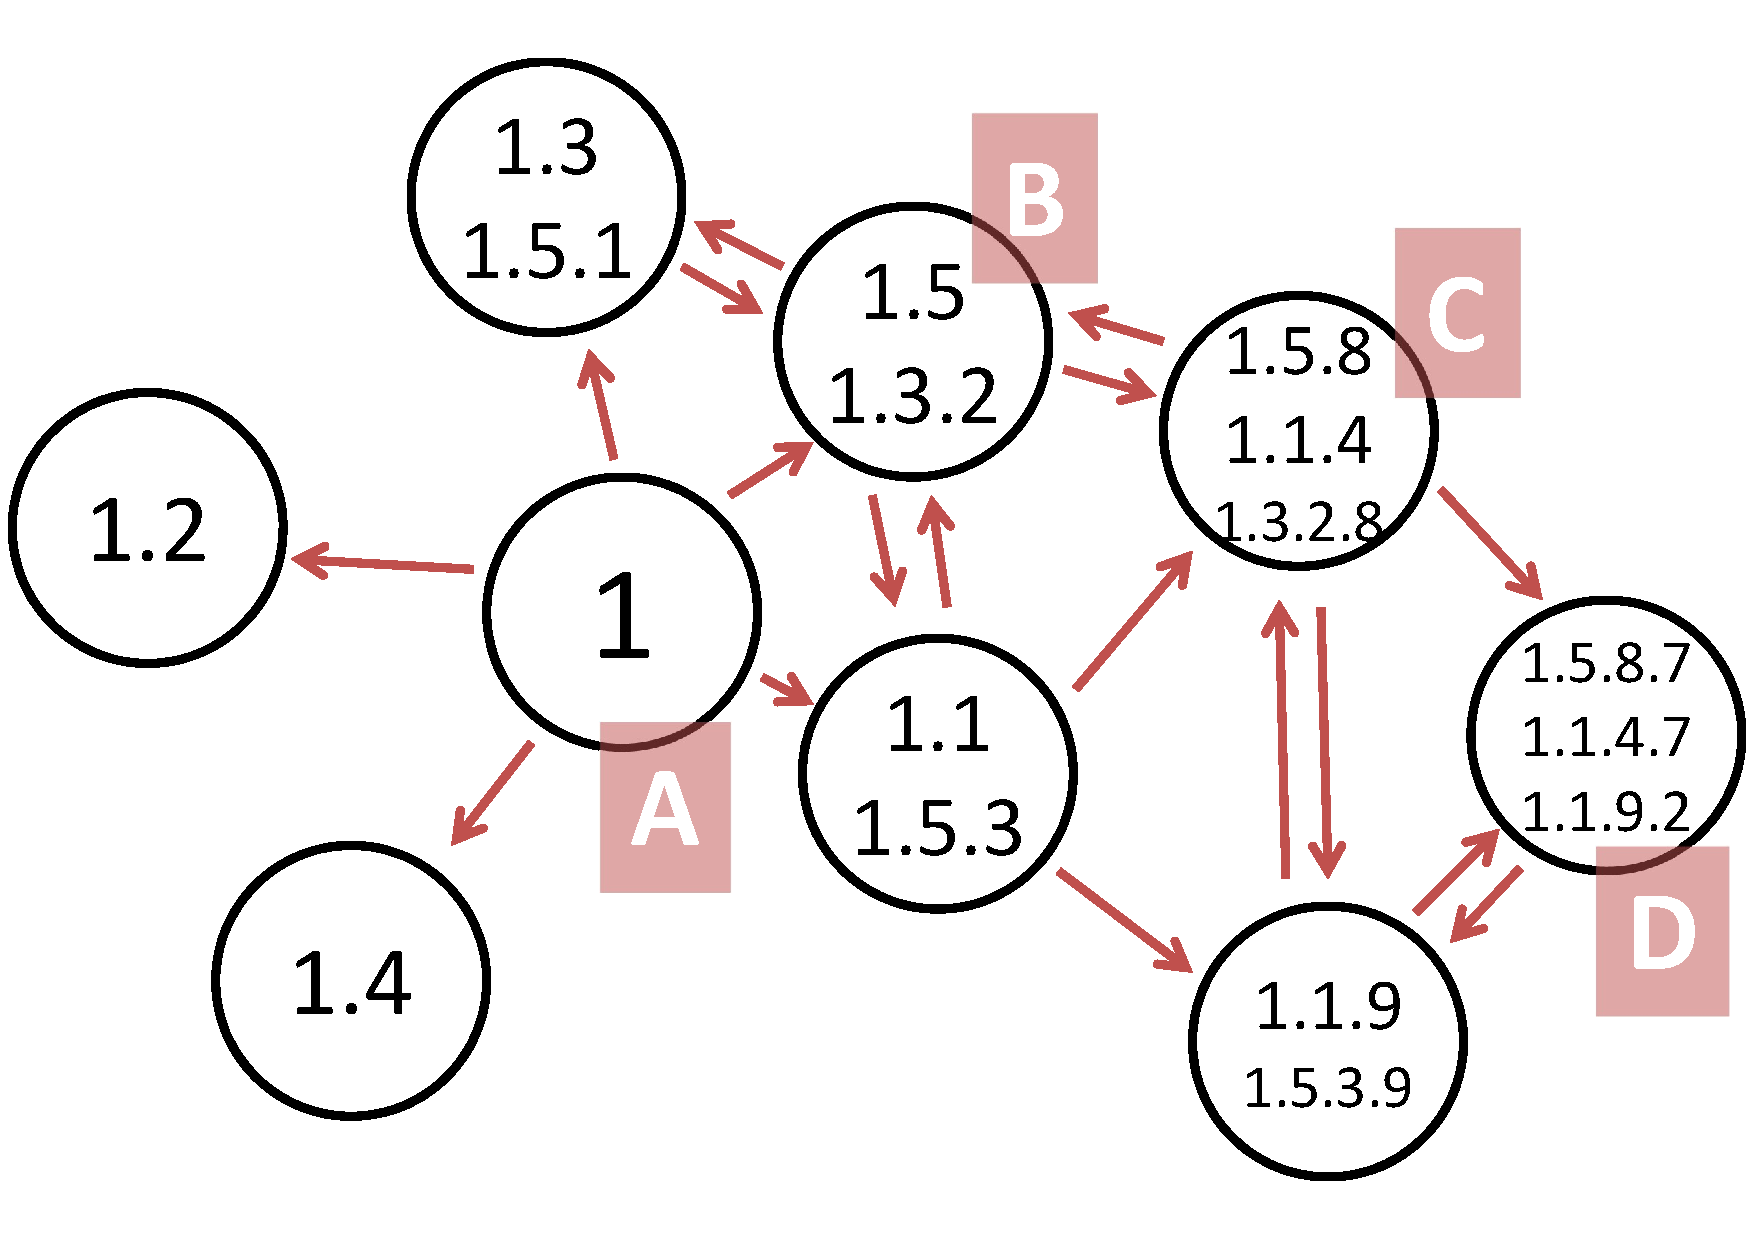
\includegraphics[width=\textwidth]{archivos/img/analisis/iotorii-operation.pdf}
    \caption{Operativa del protocolo de IoTorii \cite{rojas2021outperforming}}
    \label{fig:iotorii-operation}
\end{figure}

\begin{algorithm}[ht!]
    \SetAlgoLined
    %\KwResult{Write here the result }
    % initialization\;
    send \textit{Hello}\;
    \While{frame received}{
        %instructions\;
        \uIf{Hello}{
            \eIf{MAC not in Hello table}{
                assign unique \textit{suffix}\;
                save tuple \{\textit{MAC,suffix}\}\;
                \If{root node}{
                    create \textit{SetHLMAC} with HLMAC=1\;
                    \For{each tuple in Hello table}{
                        add tuple to \textit{SetHLMAC}\;
                    }
                    broadcast \textit{SetHLMAC}\;
                }
            }{
                discard\;
            }
        }
        \uElseIf{SetHLMAC}{
            \eIf{HLMAC (or prefix) not in HLMAC table}{
                save HLMAC in \textit{HLMAC table}\;
                create \textit{SetHLMAC} with received HLMAC\;
                \For{each tuple in Hello table}{
                    add tuple to \textit{SetHLMAC}\;
                }
                broadcast \textit{SetHLMAC}\;
            }{
                discard\;
            }
        }
        \Else{
            discard\;
        }
    }
    \caption{Assignment of HLMACs in IoTorii}
    \label{iotorii-alg}
\end{algorithm}

\begin{figure}[ht!]
    \centering
    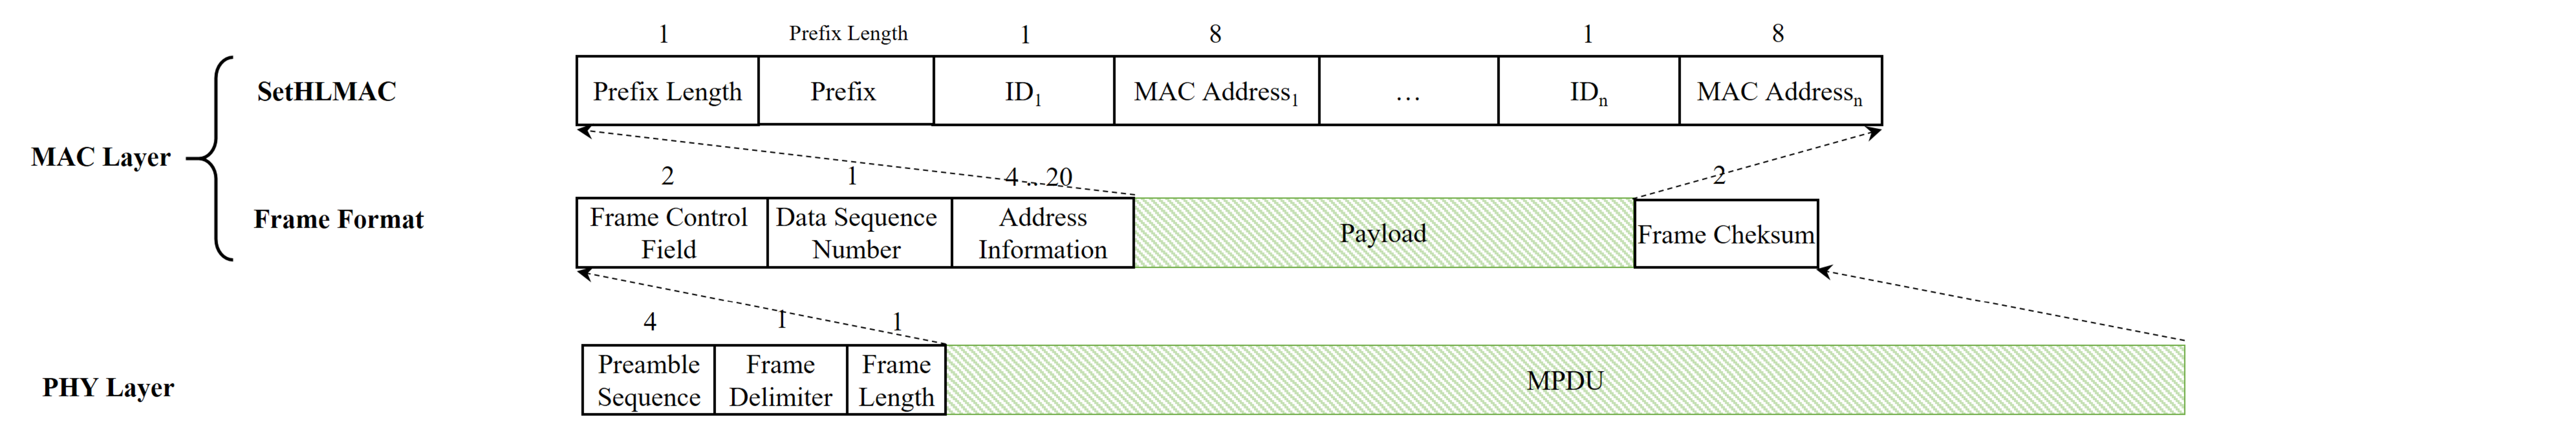
\includegraphics[width=\textwidth]{archivos/img/analisis/Comparation_frame_iotorii.eps}
    \caption{Mensajes de control en IoTorii \cite{rojas2021outperforming}}
    \label{fig:frameformat-setHLMAC}
\end{figure}

%%%%%%%%%%%%%%%%%%%%%%%%%%%%%%%%%%%%%%%%%%%%%%%%%%%%%%%%%%%%%%%%%%%%%%%%%%%%%%%%%%%%%%%%%%%%%%%%%
\section{Plataforma de desarrollo y validación}
\label{sec:ana_mininet_wifi}

blabla bla contikiwith cooja vs mininet wifi (sim vs emu )

%%%%%%%%%%%%%%%%%%%%%%%%%%%%%%%%%%%%%%%%%%%%%%%%%%%%%%%%%%%%%%%%%%%%%%%%%%%%%%%%%%%%%%%%%%%%%%%%%
\section{Agente \glsentryshort{sdn}}
\label{sec:ana_switch}

why bofuss ? i mean, we have already an implementation of inband on it

\dots

%%%%%%%%%%%%%%%%%%%%%%%%%%%%%%%%%%%%%%%%%%%%%%%%%%%%%%%%%%%%%%%%%%%%%%%%%%%%%%%%%%%%%%%%%%%%%%%%%
\section{Agente de control \glsentryshort{sdn}}
\label{sec:ana_controller}

En este punto se tiene que valorar qué agente de control \gls{sdn}, es decir controlador \gls{sdn} se va a utilizar. Se tendrán en cuenta las condiciones del entorno sobre el cual se va a desplegar, así como las características propias de cada controlador, así como la facilidad y flexibilidad que nos entregue cada uno para desplegarlo sobre la plataforma emulada. Las opciones que se han considerado para este cometido son las siguientes:

\begin{itemize}
    \item Ryu, explicado anteriormente en la sección \ref{subsec:ryu} del estado del arte.

    \item \gls{onos}, explicado anteriormente en la sección \ref{subsec:ONOS} del estado del arte.
\end{itemize}

Según se ha explicado ya, cada herramienta tiene sus puntos fuertes y sus puntos debiles, por lo que vamos a realizar una comparativa para nuestro caso de uso para ver cual de las dos nos interasa mś utilizar para este proyecto.

\begin{itemize}
    \item El controlador ONOS es más potente que Ryu, es utilizado generalmente por los operadores de red, y es conocido por su rendimiento y su solided.
    \item El controlador ONOS tiene un rendimiento superior a Ryu en terminos de procesamiento de paquetes.
    \item El controlador Ryu sin embargo, pesa menos, y es más sencillo de depurarle y meter nuevas funcionalidades si es necesario.
    \item El controlador Ryu al pesar menos, tambien se despliega y se instala más rapido frente al controlador de ONOS.
    \item Al ser más Ryu más pequeño, la curva de aprendizaje de ryu frente a ONOS también es menor.
    \item Una cosa que sería una ventaja es que ONOS tiene descubrimiento topologico con una interfaz web bastante fancy que nos ayudaría a depurar el código desarrollado del protocolo, sin embargo, esta aplicación de descubrimiento topologico corre haciendo uso del protocolo \gls{lldp}, el cual no decubriría la configuración de los enlaces inalambricos, solo a los nodos, por lo que no seria de utilidad. Si bien es cierto que hay algunas publicaciones que si han contemplado esta necesidad, sería inviable poner a implementar dicho protocolo en el proyecto dado que se escaparía de los objetivos temporales y de alcance del proyecto.
\end{itemize}

%%%%%%%%%%%%%%%%%%%%%%%%%%%%%%%%%%%%%%%%%%%%%%%%%%%%%%%%%%%%%%%%%%%%%%%%%%%%%%%%%%%%%%%%%%%%%%%%%
\section{Análisis funcional de la interfaz del \glsentryshort{bofus}}
\label{sec:ana_bofuss}

En esta sección, exploraremos en detalle el análisis funcional de la interfaz del \gls{bofus}, centrándonos específicamente en los binarios que componen su arquitectura. Estos binarios, conocidos como \texttt{ofdatapath} y \texttt{ofprotocol}, desempeñan un papel fundamental en la operativa básica de este switch de espacio de usuario.\\
\\
El \texttt{ofdatapath}, como su nombre sugiere, es responsable de procesar el plano de datos en el \gls{bofus}. Este componente se encarga de recibir, analizar y tomar decisiones en función de los paquetes que atraviesan su pipeline de procesado de paquetes. A través del parser, tablas de flujo, y tablas de métricas, el ofdatapath garantiza una transferencia de datos fluida y eficiente en el entorno OpenFlow. Por otro lado, el \texttt{ofprotocol} se ocupa del agente de control en el \gls{bofus}. Su función principal consiste en establecer la comunicación entre el controlador y el switch. A través del \texttt{ofprotocol}, el controlador y \gls{bofus} pueden intercambiar información sobre el estado del switch, enviar nuevas reglas de procesado de paquetes, o recopilar estadísticas. Este binario es quien habilita al controlador llevar a cabo una gestión centralizada y dinámica de las políticas de red, facilitando la adaptación y optimización de la infraestructura según las necesidades del entorno.\\


\subsection{Binario \texttt{ofprotocol}}

El binario de ofprotocol establece un canal seguro de comunicación entre el \textit{datapath} OpenFlow y el controlador remoto. Este conecta con el plano de datos mediante Netlink o TCP, y con el controlador remoto mediante TCP o SSL, actuando de proxy entre los dos mundos. Se quiere señalar el hecho de que el binario pueda comunicarse con el \textit{datapath} mediante TCP, dado que según el creador de la herramienta indica que esos dos binarios pueden trabajar desacoplados en máquinas diferentes y comunicarse a través de la red. Sin embargo, esta configuración no es muy común, dado que la comunicación entre \textit{datapath} y agente de control es crítica, y no admiten ni delays, ni perdidas.\\


\begin{lstlisting}[language= bash, style=Consola, caption={Interfaz CLI del binario ofprotocol},label=code:binofproto]
    ofprotocol [options] datapath controller[,controller...]
\end{lstlisting}
\vspace{0.5cm}

Uno de los parámetros obligatorios a la hora de invocar al agente de control, es qué \textit{datapath} se va a gestionar. Este se puede indicar de las siguientes formas.

\begin{itemize}
    \item \texttt{unix:file}, se indica un descriptor de un socket UNIX, el cual deber ser el mismo que se indique a la hora que ejecute el ofdatapath. Mediante este socket unix se comunicarán \textit{datapath} y agente de control.

    \item \texttt{tcp:HOST[:PORT]}, en este caso, también se puede conectar en red mediante puerto y dirección IP. Este tipo de identificación se usa cuando se quiere tener separado en máquinas diferentes \textit{datapath} y agente de control. El puerto que se emplea por defecto es el 6653.
\end{itemize}

En cambio, el parámetro del controlador es opcional, y solo soporta conexiones TCP. Para la conexión con el controlador se contemplan dos paradigmas diferentes para la conexión del controlador.

\begin{itemize}
    \item \texttt{out-of-band}: con esta configuración el tráfico OpenFlow utiliza una red privada para comunicarse con el controlador.

    \item \texttt{in-band}: con esta configuración el tráfico OpenFlow viaja por la misma red que la red de datos. Esta opción es la opción por defecto.
\end{itemize}

Para llevar a cabo la configuración manual del control in-band, es necesario realizar algunos pasos clave con antelación. En primer lugar, se requiere especificar la ubicación precisa del controlador al llamar al binario de ofprotocol. Esto asegurará una conexión adecuada entre el controlador y el agente de control. Además, es crucial configurar la interfaz de red como el puerto local OpenFlow, el cual permite que ofprotocol establezca una conexión efectiva con el controlador. El puerto local OpenFlow es un puerto de red virtual que actúa como puente entre los puertos físicos del switch y el controlador. Para lograr esto, se puede especificar el nombre de la interfaz de red asignada al puerto local mediante la opción \texttt{--local-port} en la línea de comandos del binario ofdatapath. Generalmente, si no se indica ninguna interfaz, será el propio binario quien genere una interfaz de tipo TUN/TAP con el nombre \texttt{tap0/tun0}. Siguiendo estos pasos, se puede configurar adecuadamente el control in-band.


\subsection{Binario \texttt{ofdatapath}}


La herramienta de ofdatapath representa una valiosa implementación en el ámbito de las datapaths OpenFlow. Esta herramienta, diseñada para funcionar en el espacio de usuario, tiene la capacidad de supervisar y gestionar una o más interfaces de red de manera eficiente. Estas interfaces actúan como canales de comunicación fundamentales a través de los cuales los paquetes de datos son transmitidos y reenviados según las políticas y reglas establecidas en las tablas de flujos (Ir a sección \ref{subsec:BOFUSS}). Gracias a esta funcionalidad, ofdatapath permite un control efectivo y granular a nivel de flujo de datos en la red, asegurando un enrutamiento adecuado y optimizado de los paquetes. Su flexibilidad y adaptabilidad a diferentes escenarios hacen de esta herramienta una elección preferida en entornos OpenFlow a la hora de hacer pruebas de concepto, donde se busca una implementación amigable y funcional de un agente OpenFlow. A continuación en el bloque de código \ref{code:binofdata} se indica la interfaz de comandos de este bibario.\\

\begin{lstlisting}[language= bash, style=Consola, caption={Interfaz CLI del binario ofdatapath},label=code:binofdata]
    ofprotocol [options] datapath controller[,controller...]
\end{lstlisting}
\vspace{0.5cm}

La combinación del binario ofdatapath junto con el binario ofprotocol da lugar a lo que se conoce como \gls{bofus} (Basic OpenFlow Software Switch), una solución integral de software switch \gls{sdn} OpenFlow. Al utilizar \gls{bofus}, se obtiene un control y gestión a bajo nivel de las interfaces de red, lo que permite una administración eficiente de los flujos de datos que atraviesan la pipeline de procesamiento del switch. Es importante destacar que, para acceder a estas interfaces de red, el binario generalmente requiere ejecutarse con privilegios de super usuario. Además, es relevante considerar la forma en la que estos binarios se comunican entre sí. Por lo general, esta comunicación se establece a través de un socket UNIX, permitiendo una conexión directa y eficiente entre ambos componentes. Sin embargo, también es posible establecer una conexión pasiva mediante TCP, ofreciendo una alternativa para la comunicación entre los binarios. Esta flexibilidad en los mecanismos de comunicación brinda opciones adaptativas y versátiles, permitiendo que \gls{bofus} se adapte a diferentes entornos y necesidades. \\
\\
A continuación, se indican algunos de los parámetros más importantes de la interfaz CLI del binario ofdatapath. Empezando por el único de ellos obligatorio, que es, cómo indicamos el punto de comunicación del plano de datos hacia el exterior, véase un agente de control, como por ejemplo el binario ofprotocol.\\

\begin{itemize}
    \item \texttt{punix:file}, escucha por una conexión en el descriptor del socket UNIX indicado.

    \item \texttt{ptcp:[port]}, escucha por conexiones TCP en el puerto determinado. Según la wiki de la herramienta, indican que el puerto por defecto es el 975, lo que en la práctica no es verdad\footnote{Se tuvo que modificar la wiki de la herramienta \url{https://github.com/CPqD/ofsoftswitch13/wiki/Ofdatapath-Manual/_history}}, es el 6653.
\end{itemize}

El valor del puerto por defecto se puede comprobar fácilmente, a continuación en las figuras \ref{fig:ofdata_1} y \ref{fig:ofdata_2}. Como se puede ver se lanza el binario de forma \textit{standalone} sobre la interfaz de loopback del sistema, y si comprobamos con la herramienta \texttt{lsof} los puertos TCP en esto de escucha en la Network namespace por defecto, se puede ver como el binario está utilizando el puerto 6653. Pero se puede ir un paso más allá, podemos ir al propio código fuente de la herramienta, y ver en que macro definen el puerto por defecto, lo cual se puede comprobar \href{https://github.com/CPqD/ofsoftswitch13/blob/master/include/openflow/openflow.h#LL75C1-L75C27}{aquí}.

%fig 1
\begin{figure}[ht]
    \centering
    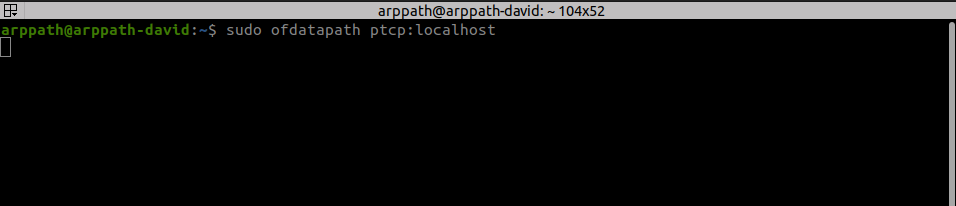
\includegraphics[width=\textwidth]{archivos/img/analisis/ofdata_1.png}
    \caption{Ejecución del binario \texttt{ofdatapath} en modo standalone}
    \label{fig:ofdata_1}
\end{figure}

%fig 2
\begin{figure}[ht]
    \centering
    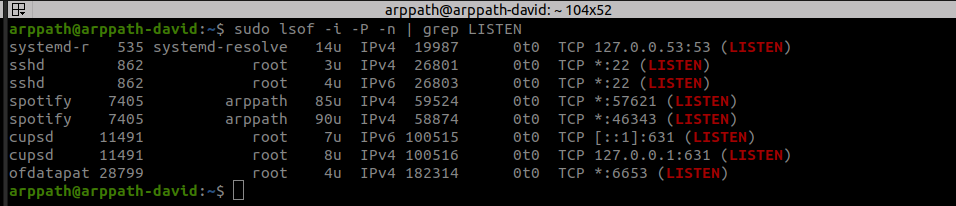
\includegraphics[width=\textwidth]{archivos/img/analisis/ofdata_2.png}
    \caption{Comprobación del puerto de  escucha del binario \texttt{ofdatapath}}
    \label{fig:ofdata_2}
\end{figure}


Sigamos con los parámetros de configuración del software switch. Uno de los más importantes, es indicar los puertos a gestionar el switch. Es decir, que interfaces va a manejar.

\begin{itemize}
    \item \texttt{-i, --interfaces=netdev[,netdev]}, Con este comando indicamos cada puerto que tendrá el switch. Cada interfaz se le asignará un número de puerto. Otro, detalle a tener en cuenta es que las interfaces no pueden tener IPs.

    \item \texttt{-L, --local-port=netdev}, Con este comando indicamos el puerto local que tendrá el switch el cual será la interfaz física o virtual, que se usará para el control in-band. Cuando está opción no está indicada, por defecto, se creará una interfaz de tipo tap, tap0 o algo así, la cual se utilizará para el control del software switch. Si no se quiere dejar como responsabilidad al Kernel la de asignar un nombre a la interfaz tap, se puede indicar como \texttt{--local-port=tap:name}. Se crea aquí. Para más información sobre las interfaces tun/tap, ver la sección \ref{linuxNetworking_tuntap}.

    \item \texttt{--no-local-port}, se le indica al software switch que no va a utilizar un puerto local, ergo, no podremos trabajar en modo in-band.

    \item \texttt{--no-slicing}, se utiliza para deshabilitar la configuración de las colas asociadas a los puertos. Por ello, contendrá un total de 0 colas. Esta opción se suele utilizar cuando algunas de las configuraciones de colas (tc y kernel) no se encuentran disponibles. (Mininet y Mininet-wifi corre el BOFUSS con esta opción por defecto).

    \item \texttt{-d, --datapath-id=dpid}, Especifica el Datapath ID Openflow, conocido como dpid. Es un identificador del datapath de 16 dígitos hexadecimales. Si no se especifica, el ofdatapath pilla uno aleatorio.
\end{itemize}

%%%%%%%%%%%%%%%%%%%%%%%%%%%%%%%%%%%%%%%%%%%%%%%%%%%%%%%%%%%%%%%%%%%%%%%%%%%%%%%%%%%%%%%%%%%%%%%%%
\section{Análisis de la clase \texttt{UserAP} en Mininet-WiFi}
\label{sec:ana_userap}

En esta sección, vamos a sumergirnos en un análisis exhaustivo de la clase \texttt{UserAP} en Mininet-WiFi, una pieza fundamental que envuelve al \gls{bofus}. Al observar detenidamente el diagrama UML de clases en la figura \ref{fig:userAP}, nos encontramos con una intrigante jerarquía de clases relacionadas con \texttt{UserAP}. En el centro de esta estructura se encuentran las clases primigenias, \texttt{Node} y \texttt{Node\_wifi}, que se llevan la mayor carga lógica al albergar la mayoría de atributos y métodos esenciales. Estas clases primigenias desempeñan un papel crucial al gestionar una serie de operaciones vitales. Entre sus responsabilidades se encuentran la creación de \textit{Network namespaces}, la configuración y creación de interfaces inalámbricas, el manejo del \gls{tc} para establecer los atributos de los enlaces y mucho más. Son el núcleo de la implementación que permite el funcionamiento armonioso de la infraestructura.\\
\\
No obstante, es importante destacar que la clase \texttt{UserAP}, encargada de encapsular al \gls{bofus}, también aporta su propia lógica especializada. Su tarea principal radica en la gestión del proceso \texttt{HostAPd}, un daemon que trabaja incansablemente para materializar las diversas funcionalidades de punto de acceso. Este componente es fundamental para dotar de vida y dinamismo a la red inalámbrica emulada. Además de su papel esencial en el despliegue del \gls{bofus}, estas clases tienen una responsabilidad adicional: implementar una interfaz de ejecución que permite adaptar las condiciones del escenario a los parámetros necesarios de la interfaz de línea de comandos del software switch \gls{sdn}. Esta adaptabilidad se convierte en una ventaja estratégica, ya que proporciona la flexibilidad necesaria para personalizar y ajustar el entorno según las necesidades específicas de cada caso de uso.
\newpage
% fig
\begin{figure}[ht!]
    \centering
    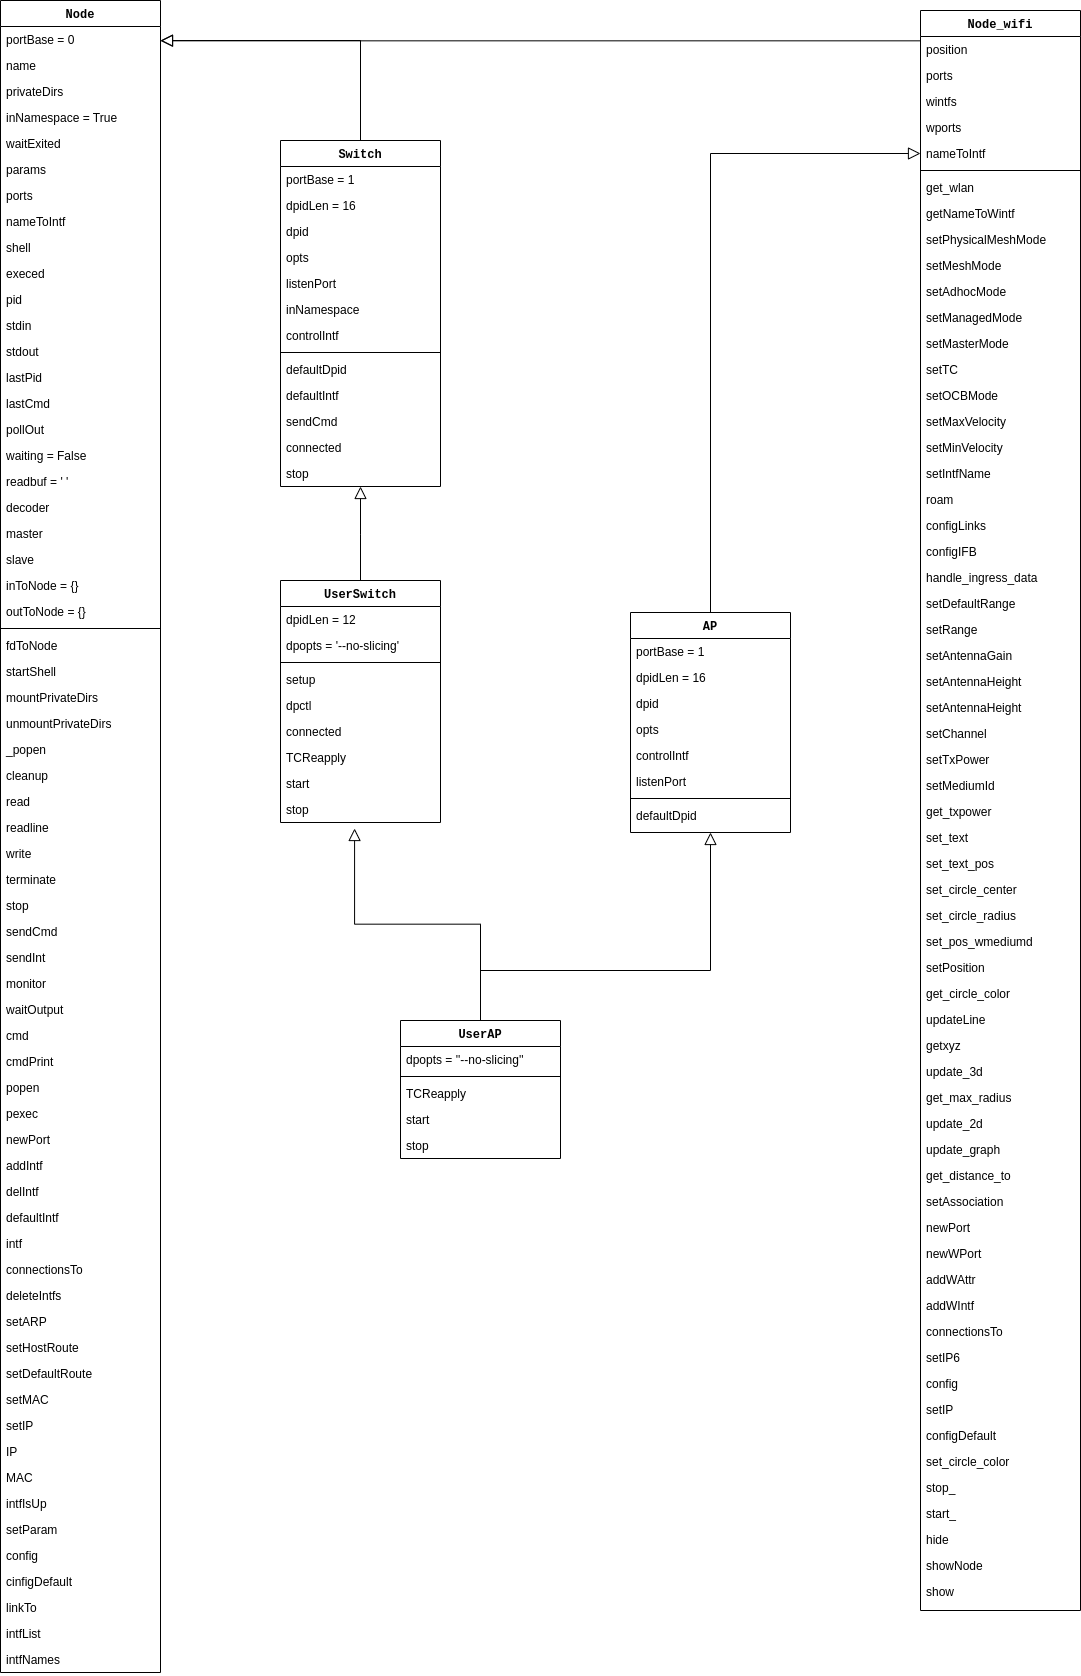
\includegraphics[width=0.8\textwidth]{archivos/img/analisis/userAP.png}
    \caption{Diagrama UML de la clase \texttt{UserAP}}
    \label{fig:userAP}
\end{figure}

Mencionar, que Mininet-Wifi redefine atributos que ya se encuentran en Mininet, como por ejemplo la longitud del identificador del \textit{datapath}. Muchos de los bugs encontrados entre los repositorios de las plataformas de emulación y el \gls{bofus}, se debe a incoherencias en la definición de las interfaces y a redefiniciones de parámetros como se ha podido encontrar. Por ello, para ver a bajo nivel como se ejecuta los binarios pertenecientes al \gls{bofus} se va a hacer una prueba de concepto lanzando una topología sencilla, y se va a estudiar las trazas de ejecución del mismo. Esto nos será de utilidad para poder comprender que comandos y llamadas al sistema se llevan a cabo para levantar una instancia de un software switch \gls{bofus}.\\
\\
La topología que se va a desplegar se puede apreciar en la figura \ref{fig:topoBasic}. Para lanzar dicha topología se tiene que lanzar un script de Python el cual se puede encontrar en el repositorio del \gls{tfm} (Sección \ref{sec:estadoArte_github}). A la par que se ejecuta el script de python que alberga la topología, se tiene que lanzar un controlador \gls{sdn} que le permita al software switch manejar correctamente los paquetes que atraviesen su \textit{datapath}. A continuación, en el bloque de código \ref{code:topoBasic}, se puede apreciar qué comandos se tienen que utilizar para  desplegar el escenario. \\

\begin{lstlisting}[language= bash, style=Consola, caption={Puesta en marcha del escenario básico},label=code:topoBasic]
    # Lanzamos el script que pone en marcha el medio inalambrico via Mininet-WiFi
    sudo python3 topo.py
   
    # Lanzamos el controlador (en otra terminal)
    ryu-manager ryu.app.simple_switch_13
\end{lstlisting}
\vspace{0.5cm}

Algún lector podría preguntarse en este punto como va a llevar se a cabo la comunicación entre el controlador \gls{sdn} y el \gls{bofus}. Dicha comunicación se producirá a través de la interfaz de red de \textit{loopback} de la Network namespace por defecto, donde el controlador de ryu estará escuchando en el puerto 6633, con una interfaz virtual de tipo \textit{tun} generada por el \gls{bofus} para llevar a cabo la conexión Openflow.  Para recolectar información sobre la traza de ejecución del script en Mininet-WiFi se debe poner el nivel de log a \textit{debug}.\\
\\

\begin{figure}[ht!]
    \centering
    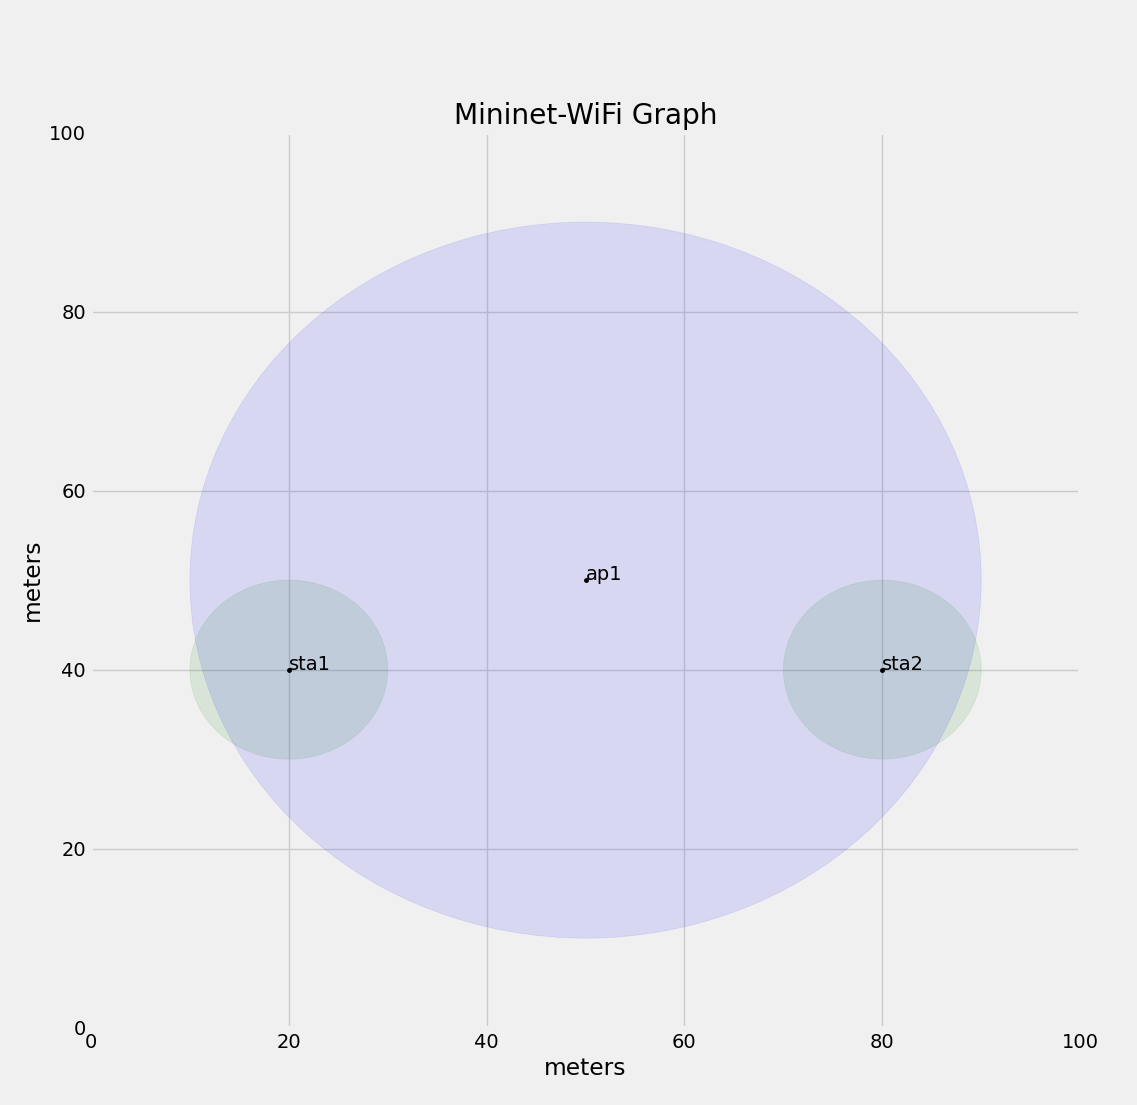
\includegraphics[width=0.7\textwidth]{archivos/img/analisis/topoBasic.png}
    \caption{Topología básica haciendo uso del \texttt{UserAP} (\gls{bofus})}
    \label{fig:topoBasic}
\end{figure}


A continuación, en el bloque de código \ref{code:trazatopobasic}, se puede apreciar la traza de ejecución de la topología básica. Dicha traza se ha limpiado y se han marcado las partes más importantes. Como se indicó anteriormente, esta traza es muy enriquecedora dado que nos permitirá a posteriori hacer nuestros propios escenarios a medida con topologías inalámbricas a bajo nivel. A lo largo de la traza, se podrán encontrar comentarios en verde que indican que operativas se están llevando a cabo en que parte.\\
\\

\begin{lstlisting}[language= bash, style=Consola, caption={Traza de la puesta en marcha del escenario básico},label=code:trazatopobasic]
    ### Primero se comprueba las caracteristicas del sistema sobre donde va a correr
    *** errRun: ['grep', '-c', 'processor', '/proc/cpuinfo'] 
    4
    0*** Setting resource limits
    *** Creating nodes
    *** Add Controller (Ryu) ***
    *** errRun: ['which', 'mnexec'] 
    /usr/bin/mnexec
    0*** errRun: ['which', 'ifconfig'] 
    /usr/sbin/ifconfig
    0_popen ['mnexec', '-cd', 'env', 'PS1=\x7f', 'bash', '--norc', '--noediting', '-is', 'mininet:c0'] 359891*** c0 : ('unset HISTFILE; stty -echo; set +m',)
    unset HISTFILE; stty -echo; set +m

    ### Se comprueba la conectividad con el controlador al puerto por defecto haciendole un telnet 
    *** c0 : ('echo A | telnet -e A localhost 6633',)
    Telnet escape character is 'A'.
    Trying 127.0.0.1...
    Connected to localhost.
    Escape character is 'A'.

    telnet> Connection closed.
    *** Add one UserAP ***
    *** errRun: ['which', 'mnexec'] 
    /usr/bin/mnexec
    0*** errRun: ['which', 'ip', 'addr'] 
    /usr/sbin/ip
    1_popen ['mnexec', '-cd', 'env', 'PS1=\x7f', 'bash', '--norc', '--noediting', '-is', 'mininet:ap1'] 359897*** ap1 : ('unset HISTFILE; stty -echo; set +m',)
    unset HISTFILE; stty -echo; set +m

    ### Se prepara el box del AP1 (El cual correrá el BOFUSS)
    added intf lo (0) to node ap1
    *** ap1 : ('ifconfig', 'lo', 'up')
    *** errRun: ['which', 'ofdatapath'] 
    /usr/local/bin/ofdatapath
    0*** errRun: ['which', 'ofprotocol'] 
    /usr/local/bin/ofprotocol

    ### Se prepara los boxes de las estaciones wifi
    *** Add two WiFi stations ***
    *** errRun: ['which', 'mnexec'] 
    /usr/bin/mnexec
    0*** errRun: ['which', 'ip', 'addr'] 
    /usr/sbin/ip
    1_popen ['mnexec', '-cdn', 'env', 'PS1=\x7f', 'bash', '--norc', '--noediting', '-is', 'mininet:sta1'] 359904*** sta1 : ('unset HISTFILE; stty -echo; set +m',)
    unset HISTFILE; stty -echo; set +m
    _popen ['mnexec', '-cdn', 'env', 'PS1=\x7f', 'bash', '--norc', '--noediting', '-is', 'mininet:sta2'] 359906*** sta2 : ('unset HISTFILE; stty -echo; set +m',)
    unset HISTFILE; stty -echo; set +m

    ### Se generan los radio taps emulados hacinedo uso del modulo del kernel mac80211_hwsim
    *** Configuring nodes
    Loading 3 virtual wifi interfaces
    Created mac80211_hwsim device with ID 0
    Created mac80211_hwsim device with ID 1
    Created mac80211_hwsim device with ID 2
    rfkill unblock 17

    ### Se cambian los nombres por defecto de las interfaces virtuales generadas a nombres 
    ### descriptivos que identifiquen a los nodos
    *** sta1 : ('ip link set wlan0 down',)
    *** sta1 : ('ip link set wlan0 name sta1-wlan0',)
    rfkill unblock 18
    *** sta2 : ('ip link set wlan1 down',)
    *** sta2 : ('ip link set wlan1 name sta2-wlan0',)
    *** ap1 : ('ip link set wlan2 down',)
    *** ap1 : ('ip link set wlan2 name ap1-wlan1',)
    *** ap1 : ('ip link set ap1-wlan1 up',)

    ### Se configura la interfaz virtual emulada wireless de la sta1
    added intf sta1-wlan0 (0) to node sta1
    *** sta1 : ('ip link set', 'sta1-wlan0', 'down')
    *** sta1 : ('ip link set', 'sta1-wlan0', 'address', '00:00:00:00:00:02')
    *** sta1 : ('ip link set', 'sta1-wlan0', 'up')
    *** sta1 : ('ip addr flush ', 'sta1-wlan0')
    *** sta1 : ('ip addr add 10.0.0.1/8 brd + dev sta1-wlan0 && ip -6 addr add 2001:0:0:0:0:0:0:1/64 dev sta1-wlan0',)
    *** sta1 : ('ip -6 addr flush ', 'sta1-wlan0')
    *** sta1 : ('ip -6 addr add', '2001:0:0:0:0:0:0:1/64', 'dev', 'sta1-wlan0')
    *** sta1 : ('ip link set lo up',)

    ### Se configura la interfaz virtual emulada wireless de la sta2
    added intf sta2-wlan0 (0) to node sta2
    *** sta2 : ('ip link set', 'sta2-wlan0', 'down')
    *** sta2 : ('ip link set', 'sta2-wlan0', 'address', '00:00:00:00:00:03')
    *** sta2 : ('ip link set', 'sta2-wlan0', 'up')
    *** sta2 : ('ip addr flush ', 'sta2-wlan0')
    *** sta2 : ('ip addr add 10.0.0.2/8 brd + dev sta2-wlan0 && ip -6 addr add 2001:0:0:0:0:0:0:2/64 dev sta2-wlan0',)
    *** sta2 : ('ip -6 addr flush ', 'sta2-wlan0')
    *** sta2 : ('ip -6 addr add', '2001:0:0:0:0:0:0:2/64', 'dev', 'sta2-wlan0')
    *** sta2 : ('ip link set lo up',)

    ### Se configura la interfaz virtual emulada wireless de la ap1 y el proceso
    ### de hostAPd
    added intf ap1-wlan1 (1) to node ap1
    *** ap1 : ('ip link set', 'ap1-wlan1', 'up')
    *** ap1 : ('ethtool -K', <WirelessLink ap1-wlan1>, 'gro', 'off')
    *** ap1 : ('ip link set', 'ap1-wlan1', 'down')
    *** ap1 : ('ip link set', 'ap1-wlan1', 'address', '00:00:00:00:00:01')
    *** ap1 : ('ip link set', 'ap1-wlan1', 'up')
    *** ap1 : ("echo 'interface=ap1-wlan1\ndriver=nl80211\nssid=new-ssid\nwds_sta=1\nhw_mode=g\nchannel=1\nctrl_interface=/var/run/hostapd\nctrl_interface_group=0' > mn359884_ap1-wlan1.apconf",)
    > > > > > > > *** ap1 : ('hostapd -B mn359884_ap1-wlan1.apconf ',)
    ap1-wlan1: interface state UNINITIALIZED->ENABLED
    ap1-wlan1: AP-ENABLED 
    *** ap1 : ('ip link set', 'ap1-wlan1', 'down')
    *** ap1 : ('ip link set', 'ap1-wlan1', 'address', '00:00:00:00:00:01')
    *** ap1 : ('ip link set', 'ap1-wlan1', 'up')

    ### Se configura la potencia y las caracteristicas intrinsecas de los enlaces 
    _popen ['mnexec', '-da', '359897', 'tc', 'qdisc', 'replace', 'dev', 'ap1-wlan1', 'root', 'handle', '2:', 'netem', 'rate', '54.0000mbit', 'latency', '1.00ms'] 360049*** ap1 : ('tc qdisc add dev ap1-wlan1 parent 2:1 handle 10: pfifo limit 1000',)
    *** sta1 : ('iw dev', 'sta1-wlan0 set txpower fixed 1400')
    *** sta2 : ('iw dev', 'sta2-wlan0 set txpower fixed 1400')
    *** ap1 : ('iw dev', 'ap1-wlan1 set txpower fixed 1400')
    *** Add links ***
    added intf sta1-wlan0 (0) to node sta1
    *** sta1 : ('ip link set', 'sta1-wlan0', 'up')
    *** sta1 : ('ethtool -K', <WirelessLink sta1-wlan0>, 'gro', 'off')
    *** executing command: tc qdisc show dev sta1-wlan0
    *** sta1 : ('tc qdisc show dev sta1-wlan0',)
    qdisc mq 0: root 
    qdisc fq_codel 0: parent :4 limit 10240p flows 1024 quantum 1514 target 5ms interval 100ms memory_limit 32Mb ecn drop_batch 64 
    qdisc fq_codel 0: parent :3 limit 10240p flows 1024 quantum 1514 target 5ms interval 100ms memory_limit 32Mb ecn drop_batch 64 
    qdisc fq_codel 0: parent :2 limit 10240p flows 1024 quantum 1514 target 5ms interval 100ms memory_limit 32Mb ecn drop_batch 64 
    qdisc fq_codel 0: parent :1 limit 10240p flows 1024 quantum 1514 target 5ms interval 100ms memory_limit 32Mb ecn drop_batch 64 
    at map stage w/cmds: ['%s qdisc add dev %s root handle 5:0 htb default 1', '%s class add dev %s parent 5:0 classid 5:1 htb rate 11.000000Mbit burst 15k']
    *** executing command: tc qdisc add dev sta1-wlan0 root handle 5:0 htb default 1
    *** sta1 : ('tc qdisc add dev sta1-wlan0 root handle 5:0 htb default 1',)
    *** executing command: tc class add dev sta1-wlan0 parent 5:0 classid 5:1 htb rate 11.000000Mbit burst 15k
    *** sta1 : ('tc class add dev sta1-wlan0 parent 5:0 classid 5:1 htb rate 11.000000Mbit burst 15k',)
    cmds: ['%s qdisc add dev %s root handle 5:0 htb default 1', '%s class add dev %s parent 5:0 classid 5:1 htb rate 11.000000Mbit burst 15k'] 
    outputs: ['', ''] 
    _popen ['mnexec', '-da', '359904', 'iwconfig', 'sta1-wlan0', 'essid', 'new-ssid', 'ap', '00:00:00:00:00:01'] 360059
    added intf sta2-wlan0 (0) to node sta2
    *** sta2 : ('ip link set', 'sta2-wlan0', 'up')
    *** sta2 : ('ethtool -K', <WirelessLink sta2-wlan0>, 'gro', 'off')
    *** executing command: tc qdisc show dev sta2-wlan0
    *** sta2 : ('tc qdisc show dev sta2-wlan0',)
    qdisc mq 0: root 
    qdisc fq_codel 0: parent :4 limit 10240p flows 1024 quantum 1514 target 5ms interval 100ms memory_limit 32Mb ecn drop_batch 64 
    qdisc fq_codel 0: parent :3 limit 10240p flows 1024 quantum 1514 target 5ms interval 100ms memory_limit 32Mb ecn drop_batch 64 
    qdisc fq_codel 0: parent :2 limit 10240p flows 1024 quantum 1514 target 5ms interval 100ms memory_limit 32Mb ecn drop_batch 64 
    qdisc fq_codel 0: parent :1 limit 10240p flows 1024 quantum 1514 target 5ms interval 100ms memory_limit 32Mb ecn drop_batch 64 
    at map stage w/cmds: ['%s qdisc add dev %s root handle 5:0 htb default 1', '%s class add dev %s parent 5:0 classid 5:1 htb rate 11.000000Mbit burst 15k']
    *** executing command: tc qdisc add dev sta2-wlan0 root handle 5:0 htb default 1
    *** sta2 : ('tc qdisc add dev sta2-wlan0 root handle 5:0 htb default 1',)
    *** executing command: tc class add dev sta2-wlan0 parent 5:0 classid 5:1 htb rate 11.000000Mbit burst 15k
    *** sta2 : ('tc class add dev sta2-wlan0 parent 5:0 classid 5:1 htb rate 11.000000Mbit burst 15k',)
    cmds: ['%s qdisc add dev %s root handle 5:0 htb default 1', '%s class add dev %s parent 5:0 classid 5:1 htb rate 11.000000Mbit burst 15k'] 
    outputs: ['', ''] 
    _popen ['mnexec', '-da', '359906', 'iwconfig', 'sta2-wlan0', 'essid', 'new-ssid', 'ap', '00:00:00:00:00:01'] 360065
    *** Build it ***
    *** Configuring nodes

    added intf sta1-wlan0 (0) to node sta1
    *** sta1 : ('ip link set', 'sta1-wlan0', 'up')
    *** sta1 : ('ethtool -K', <WirelessLink sta1-wlan0>, 'gro', 'off')

    added intf sta2-wlan0 (0) to node sta2
    *** sta2 : ('ip link set', 'sta2-wlan0', 'up')
    *** sta2 : ('ethtool -K', <WirelessLink sta2-wlan0>, 'gro', 'off')
    *** Start the controller ***
    *** Set controllers ***

    ### AQUÍ se lanza finalmente el BOFUSS
    *** ap1 : ('ofdatapath -i ap1-wlan1 punix:/tmp/ap1 -d 100000000001 --no-slicing 1> /tmp/ap1-ofd.log 2> /tmp/ap1-ofd.log &',)
    [1] 360070
    *** ap1 : ('ofprotocol unix:/tmp/ap1 tcp:localhost:6633 --fail=closed  --listen=punix:/tmp/ap1.listen 1> /tmp/ap1-ofp.log 2>/tmp/ap1-ofp.log &',)
    *** RUN Mininet-Wifis CLI ***
    *** Starting CLI:
    *** errRun: ['stty', 'echo', 'sane', 'intr', '^C'] 
\end{lstlisting}
\vspace{0.5cm}

De esta traza se quiere destacar, aparte de la gestión que lleva a cabo con las interfaces inalámbricas que se ha ido comentando a lo largo de la traza, es la ejecución de los binarios pertenecientes al software switch \gls{bofus}, \texttt{ofdatapath} y el \texttt{ofprotocol}. A continuación en el bloque \ref{code:bofussLaunch}, se dejan las líneas extraídas del bloque anterior.\\
\\

\begin{lstlisting}[language= bash, style=Consola, caption={Puesta en marcha del BOFUSS},label=code:bofussLaunch]
    # Binario del datapath 
    ofdatapath -i ap1-wlan1 punix:/tmp/ap1 -d 100000000001 --no-slicing 1> /tmp/ap1-ofd.log 2> /tmp/ap1-ofd.log 
   
    # Binario del agente de control
    ofprotocol unix:/tmp/ap1 tcp:localhost:6633 --fail=closed  --listen=punix:/tmp/ap1.listen 1> /tmp/ap1-ofp.log 2>/tmp/ap1-ofp.log 
\end{lstlisting}
\vspace{0.5cm}

Según se ha estudiado en la sección anterior \ref{sec:ana_bofuss} donde se ha estudiado la interfaz CLI del \gls{bofus}, podemos llegar a entender cada parámetro que Mininet-WiFi mediante la clase \texttt{UserAP} ha conseguido traducir del script de la topología básica a la llamada de los dos binarios del software switch.  De las dos llamadas a cada binario, se quiere mencionar que Mininet-WiFi por defecto suele mandar los logs del plano de datos y del agente de control al directorio temporal (\texttt{/tmp/}) de la distribución linux en cuestión, pero no solo los archivos de logs, también se ubican ahí los descriptores de archivos UNIX para intercomunicar \texttt{ofdatapath} y el \texttt{ofprotocol}.


%%%%%%%%%%%%%%%%%%%%%%%%%%%%%%%%%%%%%%%%%%%%%%%%%%%%%%%%%%%%%%%%%%%%%%%%%%%%%%%%%%%%%%%%%%%%%%%%%
\section{Análisis del entorno de depuración del \glsentryshort{bofus}}
\label{sec:ana_gdb}

En esta sección, exploraremos el proceso de depuración del \gls{bofus} utilizando Visual Studio Code (VS Code) y los conocimientos adquiridos sobre el funcionamiento de la interfaz de línea de comandos  del \gls{bofus} en Mininet-WiFi (Ver sección \ref{sec:ana_bofuss}). El objetivo es comprender en detalle cómo se ejecutan los comandos y qué sucede internamente durante la operación del \gls{bofus} en un entorno de red inalámbrica emulada. En nuestro escenario, trabajaremos con Mininet-WiFi, que nos proporciona un entorno virtualizado para la emulación de redes inalámbricas gracias al modulo del Kernel mac80211\_hwsim. Por ello, trabajaremos en estrecha colaboración con Mininet-WiFi para llevar a cabo la depuración. Sin embargo, este enfoque puede presentar cierta complejidad, por lo que realizaremos una primera aproximación ejecutando el código de una topología sencilla en modo de depuración, lo que nos permitirá observar los comandos que se ejecutan y comprender su funcionamiento. Posteriormente, exploraremos cómo convertir estos comandos en scripts de shell para mayor conveniencia y automatización. Nuestras herramientas de trabajo serán las siguientes:\\

\begin{itemize}
    \item Visual Studio Code (VS Code): Utilizaremos este editor para escribir y editar el código, así como para realizar la depuración paso a paso. VS Code proporciona una interfaz intuitiva y funciones avanzadas de depuración que nos facilitarán el proceso. A parte de tener una maravillosa terminal integrada y una interfaz con GDB ya desarrollada.

    \item Mininet-WiFi: Esta herramienta nos permitirá emular redes inalámbricas. Trabajaremos con una topología específica, la cual ya hemos mencionado en la sección anterior, y la ejecutaremos en modo de depuración para comprender mejor su funcionamiento, para así poder extraer las lineas de comandos necesarias para replicar su funcionamiento de forma completamente externa.

    \item GDB: Utilizaremos el depurador GDB para analizar y depurar el código del BOFUSS. GDB nos permitirá examinar el estado del programa en tiempo de ejecución, establecer puntos de interrupción, inspeccionar variables y ejecutar el código paso a paso, lo que nos ayudará a identificar posibles errores y problemas en el BOFUSS.
\end{itemize}

Por tanto, vamos a resumir que estrategia vamos a seguir para depurar al switch. Según se puede apreciar en la figura \ref{fig:debugBOFUSS}, los pasos que se van a seguir para conseguir depurar al \gls{bofus} son los siguientes. Como se ha indicado, se va a utilizar la misma topología descrita en la sección \ref{sec:ana_userap}, de las cual se va a obtener la traza de ejecución de la misma. Una vez que se tiene la traza de ejecución de la misma, se desarrrollan dos shell script para levantar el escenario y otro para destruirlo. La idea destras de esto, es que podamos externalizar el proceso de levantar la topología. Si los scripts son capaces de replicar el funcionamiento de Mininet-WiFi, pasaremos a la siguiente fase, donde se configura el depurador de C que se prefiera, en nuestro caso trabajaremos con GDB. Una vez configurado en VS Code, lanzaremos la el escenario con los scripts previamente programados, y se depurará el funcionamiento del software switch.

\newpage

\begin{figure}[ht!]
    \centering
    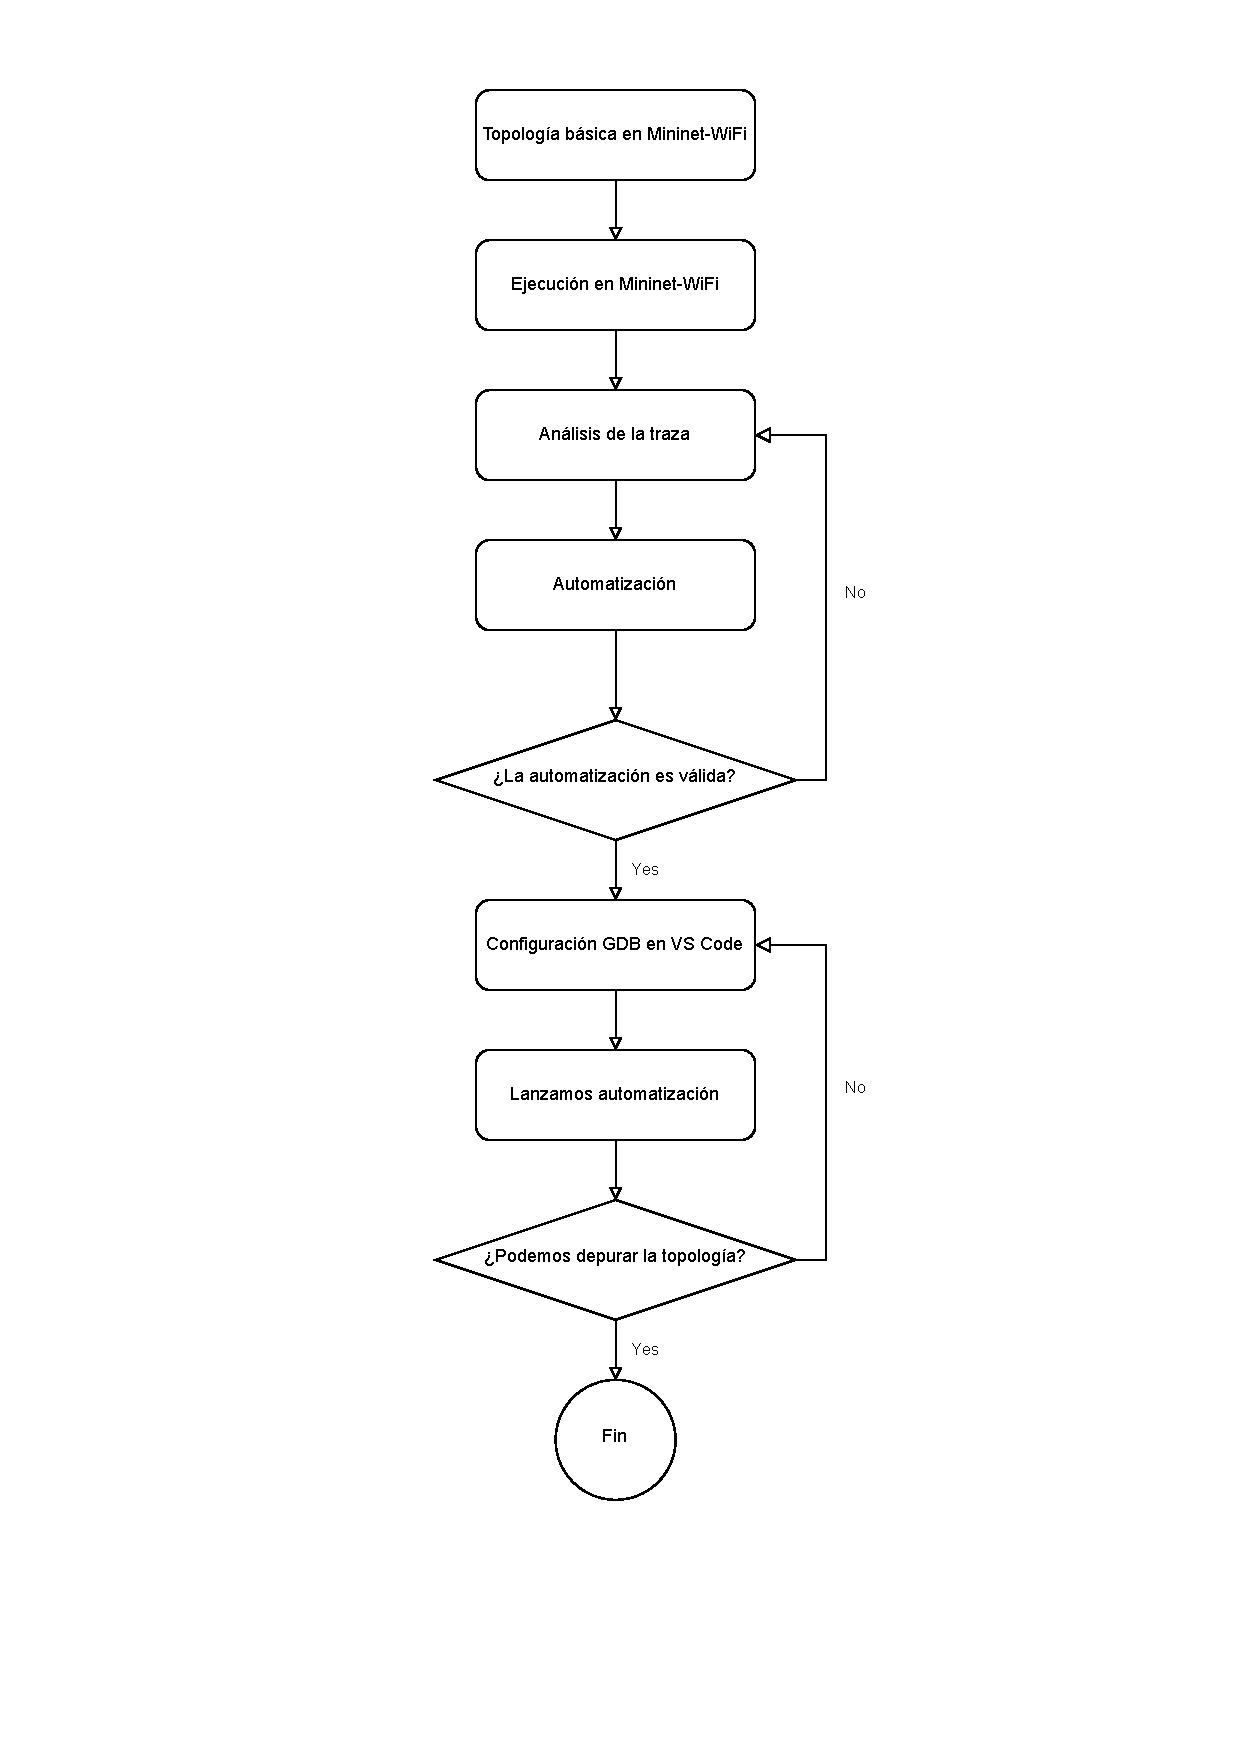
\includegraphics[width=0.9\textwidth]{archivos/img/analisis/debugBOFUSS.drawio.pdf}
    \caption{Proceso de debug al \glsentryshort{bofus}}
    \label{fig:debugBOFUSS}
\end{figure}

\subsection{Limpieza del escenario}

La limpieza del escenario es un proceso muy importante dado que la emulación de todos los escenarios que vayamos lanzando se pueden quedar en nuestro equipo haciendo que se consuman recursos o incluso arrojando un comportamiento no esperado haciendo que las conclusiones sobre los desarrollos bajo test sean incorrectos. Para la limpieza del escenario solo hará falta lanzar el siguiente script que únicamente tiene una línea de código (Ver bloque \ref{code:clean}).\\

\begin{lstlisting}[language= bash, style=Consola, caption={Script de limpieza del escenario - clean.sh},label=code:clean]
    # Lanzamos el script de limpieza del propio Mininet
    sudo mn -c
\end{lstlisting}
\vspace{0.5cm}


La simplicidad del script de limpieza es una de sus principales fortalezas. Aunque pueda parecer básico, este script ha sido probado exhaustivamente en una amplia variedad de configuraciones y topologías, demostrando su eficacia para limpiar de forma completa y agnóstica de la topología todos los componentes relacionados con la interfaz wireless.\\
\\
Durante las pruebas realizadas, en una de ellas, se han ejecutado manualmente los comandos para levantar de forma individual la interfaz wireless para el punto de acceso AP1. En este proceso, se ha observado que el script de limpieza elimina correctamente todas las configuraciones previamente establecidas con nuestro shell script. ¿Cuál es el secreto detrás de esta efectividad?\\
\\
Aquí es donde debemos reconocer el trabajo de Ramon Fontes y su contribución en el desarrollo de Mininet-WiFi. Al examinar el contenido\footnote{\href{https://github.com/intrig-unicamp/mininet-wifi/blob/master/mn_wifi/clean.py\#L77}{mininet-wifi/blob/master/mn\_wifi/clean.py-L77}} de la ruta \texttt{/sys/kernel/debug/ieee80211}, se puede encontrar una lista de todas las interfaces inalámbricas emuladas cargadas en el sistema. Es gracias a esta información que el script de limpieza puede identificar y eliminar de manera precisa todas las configuraciones relacionadas con las interfaces wireless, garantizando una limpieza completa. Como se puede ver en la figura \ref{fig:debugBOFUSS_1}, cuando se lanza el escenario topo.py, al listar las interfaces de la misma forma que lo hace Mininet-WiFi somos capaces de listar todas las interfaces inalámbricas emuladas del sistema, tanto las lanzadas desde Mininet-WiFi como las añadidas a mano haciendo uso de un shell script en paralelo.

\newpage

% fig
\begin{figure}[ht!]
    \centering
    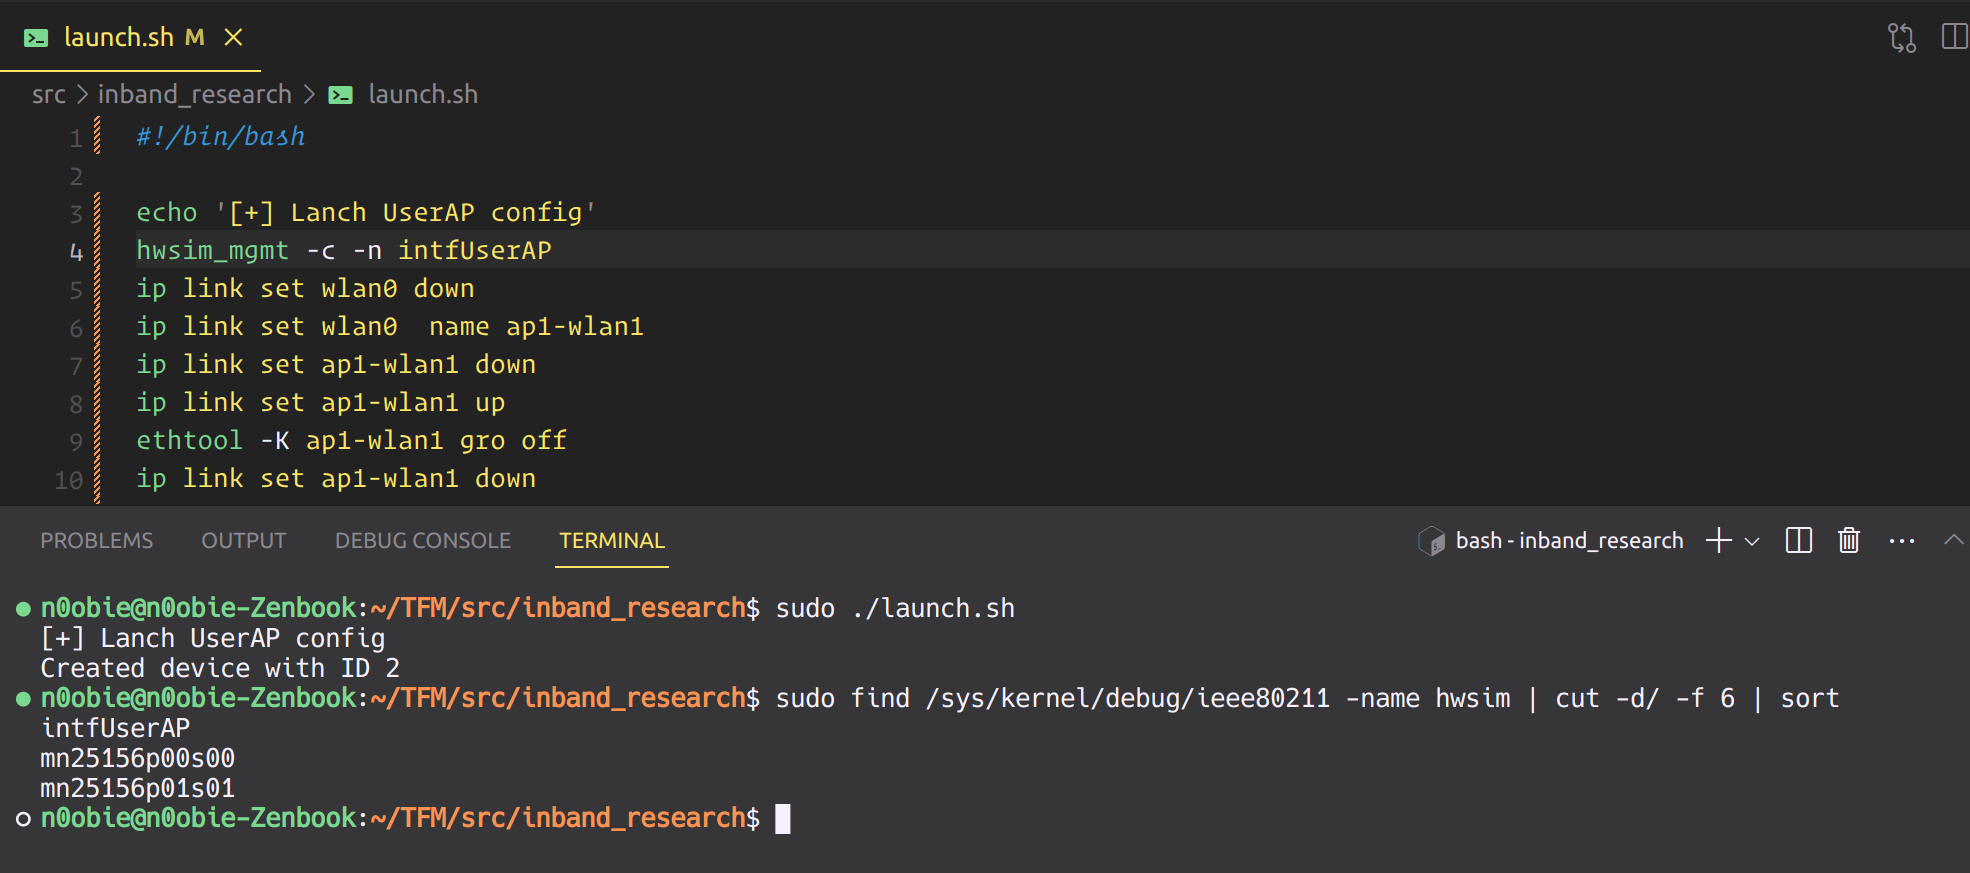
\includegraphics[width=\textwidth]{archivos/img/analisis/debugBOFUSS_1.png}
    \caption{Listado de interfaces inalámbricas en \texttt{/sys/kernel/debug/ieee80211}}
    \label{fig:debugBOFUSS_1}
\end{figure}


Como se puede ver,  como el módulo de limpieza de Mininet-WiFi lee de una ruta desde la cual listan todas las interfaces inalámbricas emuladas, cuando lancemos dicho comando, se listará nuestra capa \textit{phy} emulada, y por ende, será capaz de limpiarla a posteriori.


\subsection{Puesta en marcha del escenario}

Durante el desarrollo del script de puesta en marcha del escenario inalámbrico emulado, se llevó a cabo una exhaustiva investigación para comprender en detalle el funcionamiento interno de la topología básica y la clase \texttt{UserAP} en Mininet-WiFi. Esta investigación fue fundamental para identificar los comandos necesarios y garantizar el correcto funcionamiento del script.\\
\\
Para lograrlo, se analizaron cuidadosamente las trazas de ejecución generadas por el software switch de \texttt{UserAP}. A través de este análisis, se pudo aislar y comprender los comandos utilizados en la creación de radios emuladas. Estas trazas proporcionaron una valiosa información sobre los pasos y procesos involucrados en la configuración de las interfaces inalámbricas. En particular, se observó que la creación de radios emuladas se gestiona mediante la herramienta \texttt{hwsim\_mgmt}. Dentro del código fuente de Mininet-WiFi, este proceso se lleva a cabo en un punto específico y crítico. Este conocimiento fue esencial para extraer los comandos necesarios y adaptarlos al script de lanzamiento del \texttt{UserAP}.\\
\\
El análisis de las trazas y la comprensión del funcionamiento interno de la clase \texttt{UserAP} permitieron obtener una visión clara de los pasos necesarios para configurar y establecer las interfaces inalámbricas emuladas en el escenario. Con esta información en mano, fue posible implementar un script de lanzamiento efectivo que automatiza el proceso y asegura que todas las configuraciones sean aplicadas de manera adecuada (Ver bloque de código \ref{code:launch}).\\

\begin{lstlisting}[language= bash, style=Consola, caption={Script de puesta en marcha del escenario -  launch.sh},label=code:launch]
    #!/bin/bash

    # Vars
    AP_SSID='new-ssid'
    AP_MAC='00:00:00:00:00:01'
    STA_2_CONN=('sta1' 'sta2')

    # Create UserAP
    echo '[+] Lanch UserAP config'
    hwsim_mgmt -c -n intfUserAP
    ip link set wlan0 down
    ip link set wlan0  name ap1-wlan1
    ip link set ap1-wlan1 down 
    ip link set ap1-wlan1 up
    ethtool -K ap1-wlan1 gro off 
    ip link set ap1-wlan1 down 
    ip link set ap1-wlan1 address ${AP_MAC}
    ip link set ap1-wlan1 up
    iw ap1-wlan1 set txpower fixed 100
    echo -e "interface=ap1-wlan1\ndriver=nl80211\nssid=${AP_SSID}\nwds_sta=1\nhw_mode=g\nchannel=1\nctrl_interface=/var/run/hostapd\nctrl_interface_group=0" > mn43736_ap1-wlan1.apconf
    hostapd -B mn43736_ap1-wlan1.apconf
    ip link set ap1-wlan1 down 
    ip link set ap1-wlan1 address ${AP_MAC}
    ip link set ap1-wlan1 up
    tc qdisc replace dev ap1-wlan1 root handle 2: netem rate 54.0000mbit latency 1.00ms
    tc qdisc add dev ap1-wlan1 parent 2:1 handle 10: pfifo limit 1000
    iw dev ap1-wlan1 set txpower fixed 1400
    ofdatapath -i ap1-wlan1 punix:/tmp/ap1 -d 100000000001 --no-slicing 1> /tmp/ap1-ofd.log 2> /tmp/ap1-ofd.log &
    ofprotocol unix:/tmp/ap1 tcp:localhost:6633 --fail=closed  --listen=punix:/tmp/ap1.listen 1> /tmp/ap1-ofp.log 2>/tmp/ap1-ofp.log &

    # Connect stations to AP
    for sta in ${STA_2_CONN[@]}
    do
        echo "[+] Connecting ${sta} to UserAP"
        PID_STA=$(ps aux | grep mininet | grep ${sta} | cut -d' ' -f7)
        echo "[+] ${sta} - Detected pid ${PID_STA}"
        nsenter --target ${PID_STA} --net iwconfig ${sta}-wlan0 essid ${AP_SSID} ap ${AP_MAC}
    done
\end{lstlisting}
\vspace{0.5cm}

Como se puede ver en el bloque de código anterior, primero configuramos lo que viene a ser todos los parámetros propios de la clase \texttt{userAP}, creación de interfaces \textit{wireless} emuladas, configuración de red, además de crear la información requerida con el punto de acceso. Y más adelante lo que se hace es conectar las estaciones WiFi del escenario previamente levantado la red creada por el punto de acceso que se acaba de levantar, accediendo en cada Network namespace de cada estación WiFi.\\
\\
Se quiere añadir un par de detalles que se cree que pueden ser de utilidad al lector en caso de que quieran replicar la depuración \gls{bofus}. Como se ha podido ver para la creación de una radio emulada se tiene que hacer uso del modulo del Kernel mac80211\_hwsim, sin embargo, si se quiere trabajar con el módulo una vez ya insertado en el Kernel tendremos que utilizar otra herramienta. Dicha herrmaienta es \texttt{hwsim\_mgmt}\footnote{\url{https://github.com/patgrosse/mac80211_hwsim_mgmt}}, y a continuación en el bloque de código \ref{code:hwsim} se indican algunos ejemplos de uso de la operativa básica de la herramienta.

\begin{lstlisting}[language= bash, style=Consola, caption={Operativa básica de la herramienta hwsim\_mgmt},label=code:hwsim]
    # Crear una radio emulada
    sudo hwsim_mgmt -c -n [phy_name]

    # Para eliminarlas, se llama a la misma herramienta, de la siguiente manera
    sudo hwsim_mgmt -x [phy_name]
\end{lstlisting}
\vspace{0.5cm}

Es necesario que para trabajar con la herramienta, \texttt{hwsim\_mgmt}, que el modulo del kernel mac80211\_hwsim esté cargado, si no lo está, no podremos crear ninguna radio nueva. En la figura \ref{fig:debugBOFUSS_2} se ilustra como podemos comprobar si el módulo está previamente cargado. En este caso, si vamos a lanzar primero el script de la topología básica en primera instancia \texttt{topo.py},  el cual ya cargará el modulo, no será necesario tener que cargarlo. Si creamos una interfaz con el modulo ya cargado podemos comprobar que se ha creado un nuevo radio de la siguiente forma (Ver figura \ref{fig:debugBOFUSS_3}).

% fig
\begin{figure}[ht!]
    \centering
    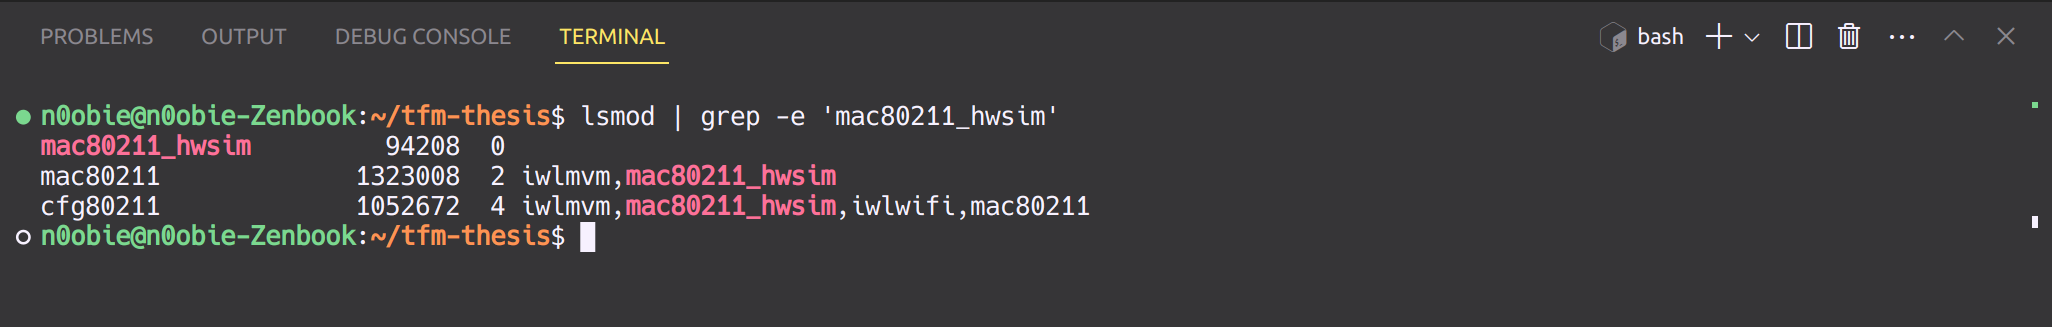
\includegraphics[width=\textwidth]{archivos/img/analisis/debugBOFUSS_2.png}
    \caption{Comprobación de si el módulo \texttt{mac80211\_hwsim} está cargado}
    \label{fig:debugBOFUSS_2}
\end{figure}

% fig
\begin{figure}[ht!]
    \centering
    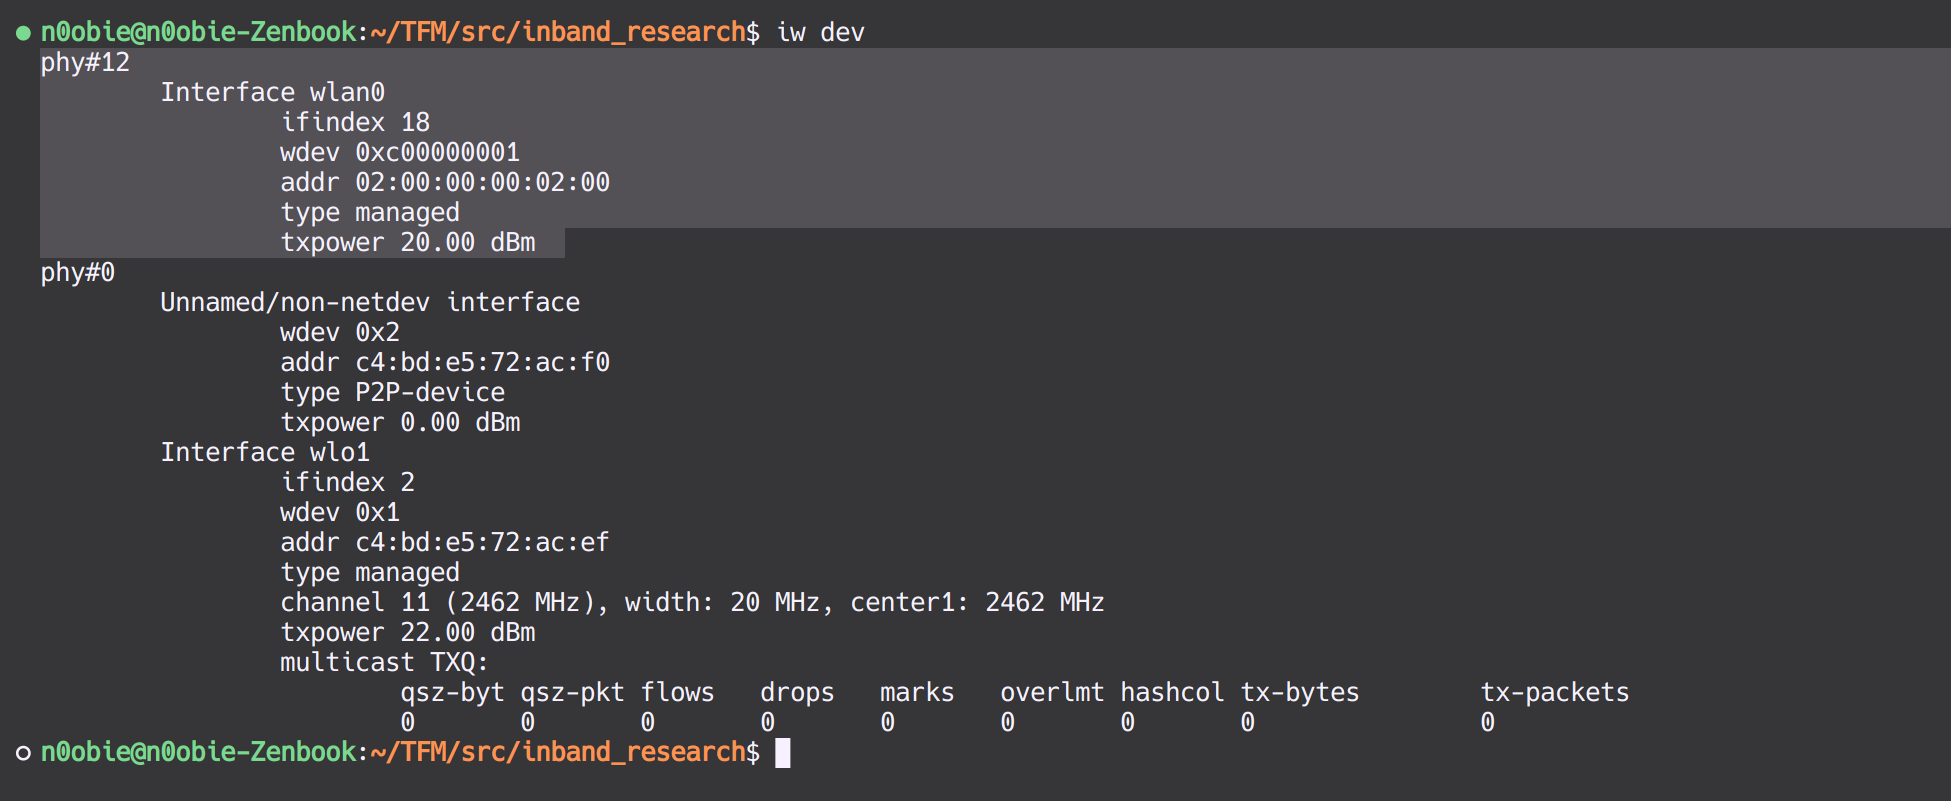
\includegraphics[width=\textwidth]{archivos/img/analisis/debugBOFUSS_3.png}
    \caption{Listado de \textit{phy} inalámbricas usando el comando \texttt{iw}}
    \label{fig:debugBOFUSS_3}
\end{figure}


\subsubsection{Troubleshooting}

Uno de los problemas más comunes que pueden surgir durante el desarrollo del escenario inalámbrico emulado, es que en algunas ocasiones, nos podemos encontrar con que la interfaz inalámbrica se bloquea y nos muestra un mensaje de advertencia indicando lo siguiente:

\begin{lstlisting}[language= bash, style=Consola, caption={Bloqueo de la interfaz por RF-Kill},label=code:rfkills1]
    ~$  Operation not possible due to RF-kill
\end{lstlisting}
\vspace{0.5cm}

Este mensaje indica que la interfaz inalámbrica está bloqueada por una restricción llamada  ``RF-kill". Esta restricción puede ser causada por diferentes factores, como un interrupción mal gestionada, una mala configuración del sistema operativo, o para salvaguardar los recursos de la máquina. Pero generalmente son \textit{soft-blocked} por el Kernel, en la mayoria de los casos para auto-protegerse. Para solucionar este problema, debemos ejecutar el siguiente comando en la terminal (Ver bloque de código \ref{code:rfkills2}).\\

\begin{lstlisting}[language= bash, style=Consola, caption={desbloqueo de la interfaz por RF-Kill},label=code:rfkills2]
    rfkill unblock all
\end{lstlisting}
\vspace{0.5cm}

Este comando desbloqueará todas las interfaces inalámbricas que estén afectadas por la restricción "RF-kill". Una vez ejecutado el comando, la interfaz inalámbrica estará disponible y podremos establecerla en el estado \texttt{UP} sin problemas.  Si el problema persiste después de ejecutar el comando mencionado, es recomendable verificar otros posibles problemas, como configuraciones incorrectas o conflictos en el sistema.

\subsection{Configuración de VS Code}

Para configurar Visual Studio Code  y poder depurar el \gls{bofus} utilizando GDB, crearemos un archivo JSON con la configuración necesaria. Antes de eso, es importante destacar que hemos logrado lanzar un escenario y ejecutar un UserAP desde un script de shell. Ahora debemos crear un archivo JSON en VS Code que invoque las dos últimas líneas de ofdatapath y ofprotocol para depurar los binarios. Por lo tanto, debemos parametrizar las instrucciones (Líneas del bloque de código \ref{code:bofussLaunch}) en el JSON de depuración. A continuación, en el bloque \ref{code:gdbjson}, se indica el JSON de configuración para la depuración.

\begin{lstlisting}[language= bash, style=Consola, caption={JSON de depuración con GDB del BOFUSS},label=code:gdbjson]
    {
        "version": "0.2.0",
        "configurations": [
            {
                "name": "(ap1)ofprotocol",
                "type": "cppdbg",
                "request": "launch",
                "program": "${workspaceFolder}/secchan/ofprotocol",
                "args": [
                    "unix:/tmp/ap1",
                    "tcp:localhost:6653",
                    "--fail=closed",
                    "--listen=punix:/tmp/ap1.listen"
                ],
                "stopAtEntry": false,
                "cwd": "${workspaceFolder}",
                "environment": [],
                "externalConsole": false,
                "MIMode": "gdb",
                "setupCommands": [
                    {
                        "text": "target-run",
                        "description": "Ofprotocol",
                        "ignoreFailures": true
                    }
                ]
            },
            {
                "name": "(ap1)ofdatapath",
                "type": "cppdbg",
                "request": "launch",
                "program": "${workspaceFolder}/udatapath/ofdatapath",
                "args": [
                    "-i",
                    "ap1-wlan1",
                    "punix:/tmp/ap1",
                    "-d",
                    "000000000001",
                    "--no-slicing"
                ],
                "stopAtEntry": false,
                "cwd": "${workspaceFolder}",
                "environment": [],
                "externalConsole": false,
                "MIMode": "gdb",
                "setupCommands": [
                    {
                        "text": "target-run",
                        "description": "Ofdatapath",
                        "ignoreFailures": true
                    }
                ]
            }
        ],
        "compounds": [
            {
                "name": "(ap1)ofprotocol/(ap1)ofdatapath",
                "configurations": [
                    "(ap1)ofprotocol",
                    "(ap1)ofdatapath"
                ],
                "preLaunchTask": "${defaultBuildTask}",
                "stopAll": true
            }
        ]
    }
\end{lstlisting}
\vspace{0.5cm}


Es importante mencionar que GDB no admite la ejecución con privilegios de root directamente. Para solucionar este problema, es necesario realizar un ajuste adicional\footnote{\url{https://github.com/microsoft/vscode-cmake-tools/issues/2463}}\footnote{\url{https://github.com/microsoft/vscode-cpptools/issues/861}}.

%%%%%%%%%%%%%%%%%%%%%%%%%%%%%%%%%%%%%%%%%%%%%%%%%%%%%%%%%%%%%%%%%%%%%%%%%%%%%%%%%%%%%%%%%%%%%%%%%
